\textit{Bearbeitet von Mohamad Shaikh Khalil}

% +++++++++++++++++++++++++++++++++++++++++++++++++++++++++++++++++
% Systemgrenzen
% +++++++++++++++++++++++++++++++++++++++++++++++++++++++++++++++++
\section{Ermittlung von Systemgrenzen / Einzuhaltende Systemgrenzen / Voraussichtliche Systemgrenzen}

\subsection*{Systemparameter}

Diese Tabelle führt die Systemparameter auf, die sich aus der vorgegebenen Anforderung von ± 0,5 mm sowie der Beschaffenheit des Systems und der gewählten Hardware ergeben haben.

\begin{table} [h]
    \centering
    \begin{tabular}{|c|c|c|c|}\hline
 parameter& symbol& value&Source\\\hline
         Teilkreisdurchmesser des Ritzels&  d&  17 mm& 	Konstruktion, m=1 d=7\\\hline
         Effektiver Radius&  r&  8.5 mm& d/2\\\hline
         Weg je umdrehung&  $s_{rev}$&  53.41 mm& \pi * d\\\hline
         Vollschritte je Umdrehung&  -&  200& 1.8°, 17HE12-1204S\\\hline
         Mikroschrittteilung&  -&  1/16& MOTOR\_MICROSTEPS\\\hline
 Weg je Vollschritt& $\Delta x vs $& 0.0267 mm&$s_{rev}$/200\\\hline
         Weg je Mikroschritt&  $q_{\mu}$&  0.0167 mm& $s_{rev}$/3200\\\hline
         Encoderauflösung&  $q_{enc}$&  0.0130mm& $s_{rev}$/4096\\\hline
         Verhältnis Motor/Encoder&  &  1.28& $\Delta x_{\mu} / \Delta x_{enc}$\\\hline
         Federsteifigkeit&  $c_{F}$&  2.12 N/mm& 2x1.06 N/m parralel\\\hline
         Rotorträgheit&  $J_{Rot}$        &4.0⋅10−6 kg m²   & Herstellerangabe\\\hline
 Bewegte Masse& $m_{bew}$        &≈ 70 g  &zahnstange + Führungsschiene\\\hline
 Motorsteifigkeit& $k_M$            & 13.0 Nm/rad &Mhalt​⋅(\pi/2)/1.8°\\ \hline
    \end{tabular}
    
    
\end{table}
%\textit{%z.B. max. Strom, Drehmoment, Geschwindigkeit, usw.}

\subsection*{Betriebsgrenzen}
\begin{table}[h]
    \centering
    \begin{tabular}{|c|c|>{\centering\arraybackslash}p{0.33\linewidth}|}\hline
         Totzone&  0.05mm&  CTRL\_DEADBAND\_MM\\\hline
         Firmware Verfahrbereich&  60mm&  CTRL\_XMIN\_MM,
CTRL\_XMAX\_MM\\\hline
         maximaler mechanischer Verfahrweg&  95mm&  Teststand\\\hline
         Laufstrom / Haltestrom&  IRUN=IHOLD=27/32&  	MotorControl\_Init()\\\hline
         Versorgungsspannung Vm&  12v&  	Stromversorgung\\ \hline
    \end{tabular}
    
    
\end{table}

Der Motorschritt und der Encoderschritt liegen relativ nahe beieinander und fallen weit unter den geforderten Bereich von ±0,5 mm. Das bedeutet, dass die Auflösung nicht der begrenzende Faktor für die Genauigkeit ist.
Da der Motorschritt größer ist als der Encoderschritt, kann der Motor nicht exakt auf dem Encoderschritt anhalten, und die daraus resultierenden Werte müssen durch eine Totzone unterdrückt werden.

Was schränkt die Genauigkeit tatsächlich ein?
\item Spiel: zwischen 0,05 und 0,1 mm, bis zu einem halben Vollschritt
\item Nichtlinearität des AS5600: ±1°, was an der Zahnstange ±0,148 mm entspricht. Dies ist der größte einzelne Faktor, der die Genauigkeit einschränkt, da der Regler meist Differenzen auswertet, die an nahezu derselben mechanischen Position gemessen werden.
\item Die Totzone

Alle drei liegen unter dem festgelegten Schwellenwert von ±0,5 mm

Referenzpunkt
Der AS5600 ist kein Absolut-Encoder und muss bei jeder Umdrehung (53,41 mm) neu referenziert werden
Die Referenz wird vom Benutzer über die Benutzeroberfläche eingestellt; für zukünftige Projektiterationen ist die Implementierung eines Referenzierungslaufs geplant

Der mechanische Verfahrbereich erlaubt bis zu 95 mm; die Beschränkung auf 60 mm reicht für die erforderlichen Aufgaben aus und dient zudem als Schutz vor einem Überschreiten der Grenzen und einem Verrutschen der Schiene

Die Kraft stellt eine Obergrenze dar.
Das Haltemoment von 260 Nmm wird bei Haltestrom (1,2 A/Phase) erreicht. Der Motor ist auf einen Betrieb bei IRUN = 27/32 eingestellt, was etwa 0,86 A entspricht – etwa 72\% des Nennstroms.
Fmax ≈ 0,72⋅260 Nmm/8,5 mm ≈ 22 N

Am Betriebspunkt von 5 N benötigt die Vorrichtung 42,5 N·mm, was 16\% des Haltemoments entspricht

% +++++++++++++++++++++++++++++++++++++++++++++++++++++++++++++++++
% Mathematisches Modell
% +++++++++++++++++++++++++++++++++++++++++++++++++++++++++++++++++
\section{Erstellung eines simplen mathematischen Modells}

Dieser Abschnitt stellt das Anlagenmodell vor, auf dem die Reglerauslegung 
sowie die Simulation basieren. Er beschreibt den Prüfstand,
nämlich eine Greiferhälfte mit einer einzelnen Zahnstange

\subsection*{Annahmen}

\begin{enumerate}
    \item \textbf{Starre Kopplung} zwischen Ritzel und Zahnstange. Das Spiel ist nicht Bestandteil
          des Systemmodells, sondern wird separat als Totzone behandelt.
    \item \textbf{Ein Freiheitsgrad.} Der Prüfstand stellt eine Greiferhälfte dar:
          ein Ritzel, eine Zahnstange.
    \item \textbf{Quasistatisches Verhalten} während des Kraftaufbaus. Die
          Begründung folgt weiter unten aus der reduzierten Trägheit.
    \item \textbf{Kein Schrittverlust.} Verifiziert durch Messung, wobei die
          Sollposition mit der gemessenen Position verglichen wird.
\end{enumerate}

\subsection*{Kinematik}

Das Ritzel rollt auf der Zahnstange, sodass Verschiebung und Drehung durch den
Steigungsradius miteinander verknüpft sind:


\begin{equation}
    x = r \cdot \varphi ,
    \qquad
    s_{rev} = \pi d = \pi \cdot 17\,\mathrm{mm} = 53,41\,\mathrm{mm}
    \label{eq:kinematik}
\end{equation}
Daraus ergeben sich die beiden Auflösungen, die den Regelkreis bestimmen:
\begin{equation}
    \Delta x_{\mu} = \frac{s_{rev}}{200 \cdot 16} = 0,0167\,\mathrm{mm} ,
    \label{eq:aufloesung_aktor}
\end{equation}

während die kleinste auflösbare Messung des Encoders mit 12 Bit pro
Umdrehung

\begin{equation}
    \Delta x_{enc} = \frac{s_{rev}}{2^{12}} = 0,0130\,\mathrm{mm} .
    \label{eq:aufloesung_encoder}
\end{equation}
Die Stellgröße des Antriebs ist eine Geschwindigkeit. Sie wird über UART in das
\texttt{VACTUAL}-Register geschrieben, woraufhin der Treiber die
entsprechenden Mikroschritte selbstständig generiert. Die Umrechnung lautet

\begin{equation}
    \texttt{VACTUAL} = k_V \cdot v ,
    \qquad
    k_V = \frac{3200 / s_{rev}}{0,71526} = 83,77\,\mathrm{(mm/s)^{-1}} ,
    \label{eq:vactual}
\end{equation}

wobei der Nenner dem internen Taktgenerator des Treibers
bei $f_{CLK} = 12$~MHz entspricht. Die Position ist das Zeitintegral der Sollgeschwindigkeit,
sodass das System ein reiner Integrator ist. Die Konsequenzen für die Reglerstruktur
werden in Kapitel 6 dargelegt.

% -----------------------------------------------------------------
\subsection*{Dynamik}

Für den einzelnen Freiheitsgrad $\varphi$ gilt der Lagrange-Formalismus mit der
kinetischen Energie

\begin{equation}
    T = \tfrac{1}{2}\left(J_{Rot} + m_{bew}\,r^2\right)\dot{\varphi}^2
    \label{eq:kinetische_energie}
\end{equation}

und der potenziellen Energie der Feder

\begin{equation}
    V = \tfrac{1}{2}\,c_{eff}\left(r\varphi - x_0\right)^2
    \qquad \text{für } x > x_0
    \label{eq:potentielle_energie}
\end{equation}

ergibt sich die Bewegungsgleichung

\begin{equation}
    \left(J_{Rot} + m_{bew}\,r^2\right)\ddot{\varphi}
    + b\,\dot{\varphi}
    + r\,c_{eff}\left(r\varphi - x_0\right)
    = M_{Motor} .
    \label{eq:bewegungsgleichung}
\end{equation}

Aufgrund der umgekehrten Führungsanordnung des Prüfstands bewegt sich die Führungsschiene
zusammen mit der Zahnstange. Die bewegte Masse umfasst daher Zahnstange und Schiene. Die reduzierte Trägheit beträgt

\begin{equation}
    J_{ges} = J_{Rot} + m_{bew}\,r^2
    = 4,0 \cdot 10^{-6} + 5,1 \cdot 10^{-6}
    \approx 9,1 \cdot 10^{-6}\,\mathrm{kg\,m^2} .
    \label{eq:traegheit}
\end{equation}

Rotor und Last tragen somit in vergleichbarem Maße dazu bei, wobei der Lastterm
eher von der Stahlführungsschiene als von der gedruckten Zahnstange dominiert wird.

% -----------------------------------------------------------------
\subsection*{Zusammenhang zwischen Weg und Kraft}

Ein Schrittmotor ist eine Positionsquelle, keine Kraftquelle. Die einzige Verbindung zwischen
Position und Kraft ist die Nachgiebigkeit des Systems: Solange sich die Zahnstange
frei bewegt, ändert sich die Position, während die Kraft null bleibt, und nach dem Kontakt wird jeder
weitere Schritt in eine Auslenkung umgewandelt:

\begin{equation}
    F =
    \begin{cases}
        c_{eff}\,(x - x_0) & \text{für } x > x_0 \\[2pt]
        0                  & \text{ansonsten}
    \end{cases}
    \label{eq:federmodell}
\end{equation}


Das Drehmoment des Ritzels ergibt sich aus der auf die einzelne Zahnstange wirkenden Kraft:

\begin{equation}
    M = F \cdot r
    \label{eq:moment_pruefstand}
\end{equation}

Im vollständigen Greifer treibt das Ritzel zwei gegenüberliegende Zahnstangen an, deren
Umfangskräfte ein Drehmoment gleicher Richtung erzeugen. Dort gilt

\begin{equation}
    M = 2 \cdot F \cdot r
    \label{eq:moment_greifer}
\end{equation}

sodass der Prüfstand den Motor nur halb so stark belastet wie es der Greifer
tun würde.

% -----------------------------------------------------------------
\subsection*{Bestimmung der beiden Parameter}

Keine der beiden Größen in Gleichung \ref{eq:federmodell} ist Teil des Modells; beide müssen
extern festgelegt werden.

Die Steifigkeit ergibt sich aus den beiden Druckfedern des Prüfstands. Diese sind
übereinander angeordnet, beide am Gestell befestigt und wirken beide gegen denselben
Anschlag. Sie erfahren daher die gleiche Verschiebung und wirken parallel:

\begin{equation}
    c_{eff} = 2 \cdot 1,06\,\mathrm{N/mm} = 2,12\,\mathrm{N/mm}
    \label{eq:steifigkeit}
\end{equation}

Dieser Wert stellt eine Obergrenze dar. Alle nachgiebigen Elemente liegen im Kraftweg
in Reihe, sodass das weichste Element dominiert:

\begin{equation}
    \frac{1}{c_{eff}}
    = \frac{1}{c_{Feder}} + \frac{1}{c_{M}} + \frac{1}{c_{Aufnahme}}
      + \frac{1}{c_{Zahnstange}} + \dots
    \label{eq:reihenschaltung}
\end{equation}

Der Motor selbst wirkt als Federelement. Bei einer magnetischen Steifigkeit von
$k_M = 13,0$~Nm/rad beträgt der äquivalente Wert an der Zahnstange

\begin{equation}
    c_{M} = \frac{k_M}{r^2} = 180\,\mathrm{N/mm} ,
    \label{eq:motorsteifigkeit}
\end{equation}

was den Gesamtwert um etwa ein Prozent senkt und daher vernachlässigbar ist
gemäß der gängigen Regel, dass Elemente, die etwa zehnmal steifer sind als das weichste
Element, vernachlässigt werden dürfen. Die PLA-Motorhalterung und die gedruckte Zahnstange sind
nach dieser Regel nicht vernachlässigbar und senken den effektiven Wert zusätzlich. Da ein
kleineres $c_{eff}$ die für eine gegebene Kraft erforderliche Durchbiegung erhöht und dadurch
die Auflösung verbessert, mit der die Kraft eingestellt werden kann.

Der Kontaktpunkt $x_0$ ist kein Konstruktionsparameter. Er muss
für jeden Greifvorgang experimentell ermittelt werden.

% ---------------------------------------------------------------
\begin{table}[h]
    \centering
    \caption{Größen des Pflanzenmodells}
    \label{tab:modellgroessen}
    \begin{tabular}{|l|l|p{6cm}|}
        \hline
        Größe & Wert & Quelle \\
        \hline
        $r$              & 8,5~mm                        & $d/2$, Konstruktionsangabe \\\hline
        $s_{rev}$        & 53,41~mm                      & $\pi d$ \\\hline
        $\Delta x_{\mu}$ & 0,0167~mm                     & \\\hline
        $\Delta x_{enc}$ & 0,0130~mm                     & \\\hline
        $k_V$            & 83,77~(mm/s)$^{-1}$           & \\\hline
        $J_{Rot}$        & $4,0 \cdot 10^{-6}$~kg\,m²    & Herstellerangaben \\\hline
        $m_{bew}$        & $\approx 70$~g                & Zahnstange, Schiene\\\hline
        $J_{ges}$        & $9,1 \cdot 10^{-6}$~kg\,m²    & \\\hline
        $k_M$            & 13,0~Nm/rad                   & $M_{halt}\cdot(\pi/2)/1,8^\circ$ \\\hline
        $c_{eff}$        & 2,12~N/mm                     & \\\hline
        $c_{M}$          & 180~N/mm                      & \\\hline
        $x_0$            & experimentell bestimmt     & \\
        \hline
    \end{tabular}
\end{table}
% ----------------- ----------------------------------------------

% -----------------------------------------------------------------
\subsection*{Geltungsbereich des Modells}

Das Modell beschreibt einen einzelnen Freiheitsgrad mit konzentrierten Parametern. Es
berücksichtigt Kinematik, Nachgiebigkeit und Trägheit, jedoch nicht die Verteilung der
Nachgiebigkeit über die Struktur, die Nichtlinearität des Getriebes oder das Kriechen unter
dauerhafter Belastung. Für das Ziel dieser Arbeit – den Nachweis, dass das System
simuliert und gesteuert werden kann – ist dieser Detaillierungsgrad ausreichend.
%\textit{Grundlage für den Reglerentwurf}


% +++++++++++++++++++++++++++++++++++++++++++++++++++++++++++++++++
% Prüfstand
% +++++++++++++++++++++++++++++++++++++++++++++++++++++++++++++++++
\section{Entwickelter Prüfstand}
\begin{figure}
    \centering
    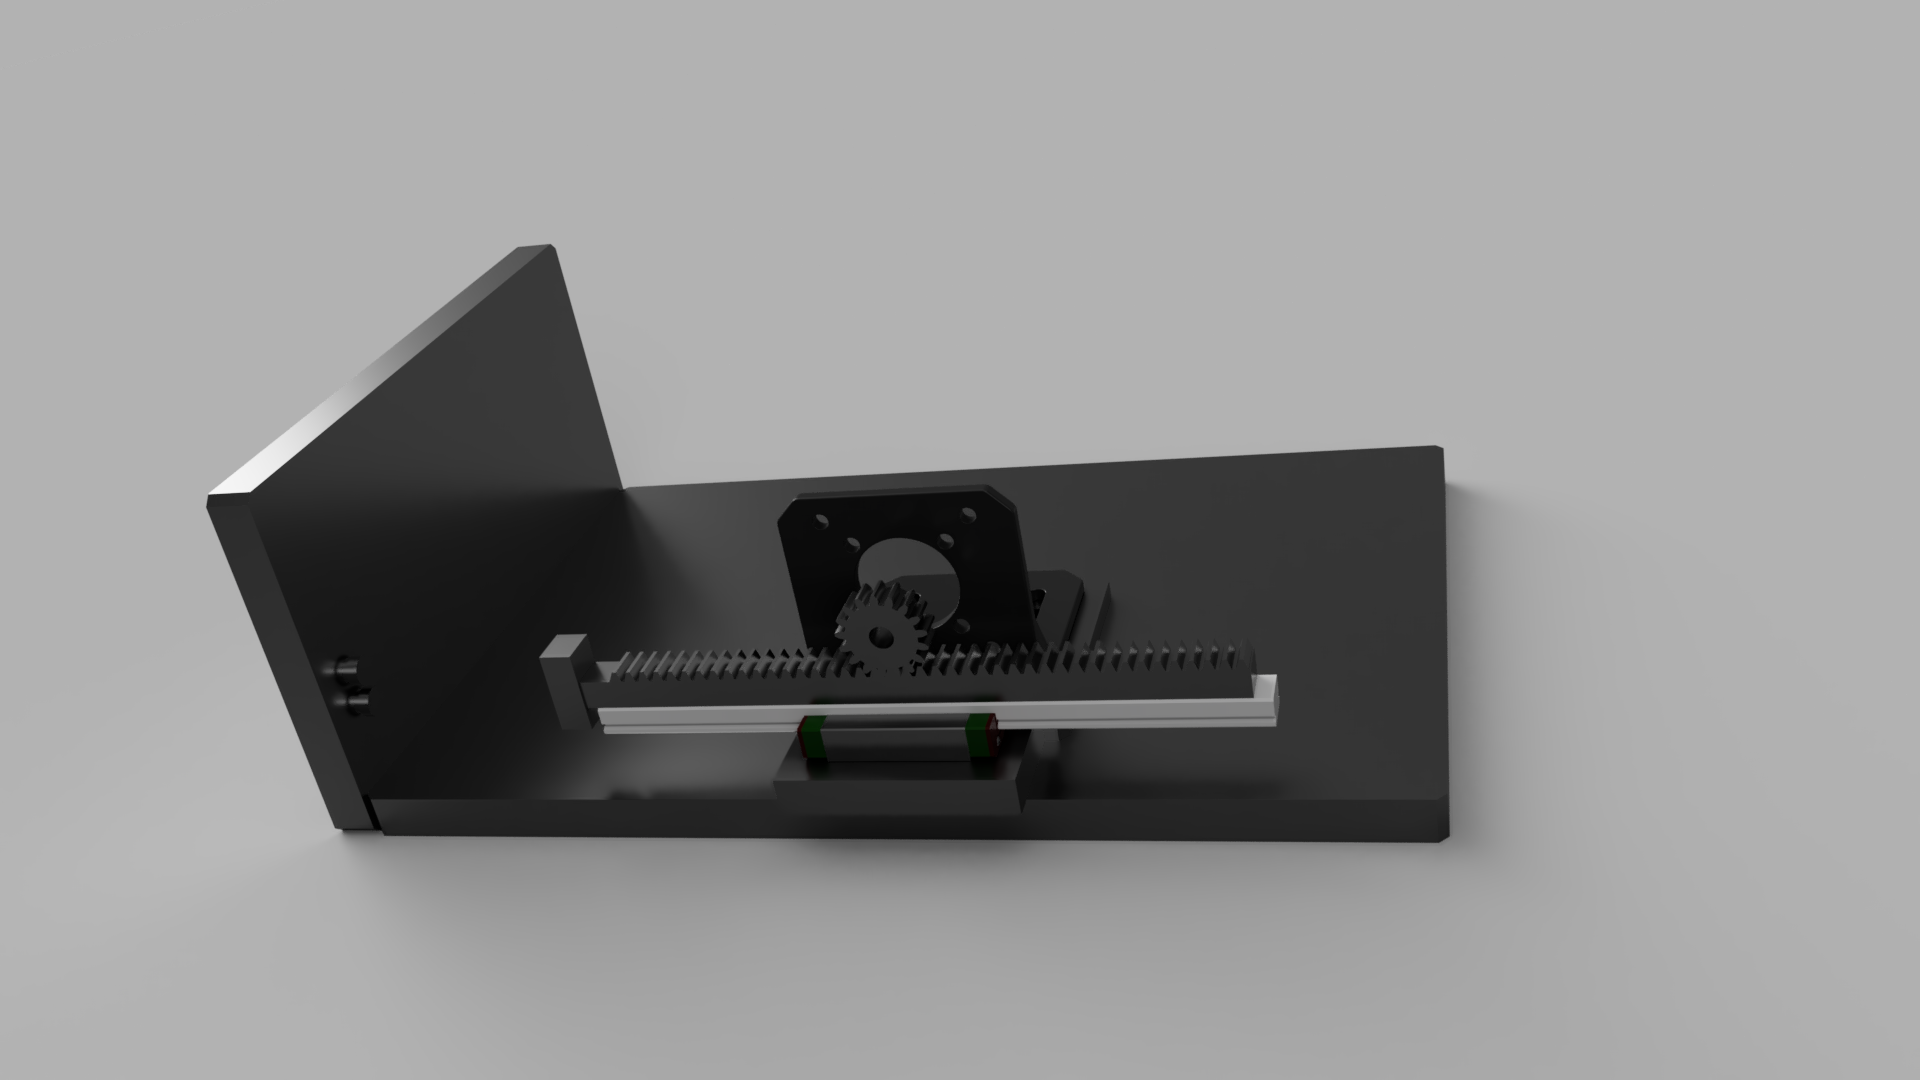
\includegraphics[width=1\linewidth]{Abbildung/dopple_feder_teststand_2026-Sep-14_05-20-54PM-000_CustomizedView4746332256.png}
    \caption{Enter Caption}
    \label{fig:Teststand}
\end{figure}
Dieses Projekt dient der Steuerung eines Endeffektors eines Roboterarms. Zuvor mussten wir jedoch die Steuerungs- und Simulationsfähigkeiten der von uns ausgewählten Komponenten und des Designs überprüfen und testen.
Aus diesem Grund wurde ein Prüfstand erstellt, um die Funktionalität des Greifers nachzubilden.

Der Prüfstand ermöglicht den Abgleich der berechneten Werte mit bekannten Parametern (Federn).

Mechanischer Aufbau
Der Prüfstand misst 240 × 85 × 150 mm. Der Motor ist auf einer Halterung montiert, die wiederum auf der Grundplatte befestigt ist.

\begin{table}
    \centering
    \begin{tabular}{|c|c|c|}\hline
         Pos.&  Komponente& Anmerkung\\\hline
         1&  Stepper motor 17HE12-1204S& seitlich an der Halterung befestigt\\\hline
 2& Motorhalterung&\\\hline
         3&  Ritzel m=1 z=17& auf der Motorwelle\\\hline
         4&  Zahnstange m =1 110mm& mit dem Ritzel verbunden\\\hline
         5&  Führungsschiene MGN9R& reist mit dem Zahnstange\\\hline
 6& Führungswagen MGN9H&an der Grundplatte befestigt\\\hline
         7&  Zwei Druckfedern mit jeweils 1,06 N/mm& am Ende der Zahnstange befestigt\\ \hline
    \end{tabular}
    
    
\end{table}
Der Schlitten, auf dem die Kugellager gelagert sind, ist an der Grundplatte befestigt, während Schiene und Zahnstange miteinander verbunden sind und sich gemeinsam bewegen. Die Schiene ist Teil der beweglichen Masse und dominiert diese (4.2). Der mechanische Hub beträgt etwa 95 mm.

Die beiden Druckfedern sind übereinander angeordnet und werden durch die Anschlagwand zusammengedrückt. Da beide die gleiche Verschiebung erfahren, addieren sich ihre Kräfte.

\textbackslash{}textbf\{Einschränkung:\} Die Motorhalterung besteht aus PLA. Aufgrund der hohen Temperatur des Motors bei längerem Betrieb kann sich die Halterung verformen. Innerhalb des Projektzeitrahmens stand kein anderes Material zur Verfügung. Für Testläufe von wenigen Sekunden Dauer ist dies unkritisch, für den Dauerbetrieb sollte die Halterung jedoch aus einem hitzebeständigeren Material bestehen.

Montage des Encoders
Der AS5600 wird an der Rückseite des Motors über eine Halterung befestigt, die den richtigen Abstand zum an der Welle angebrachten Magneten (2 mm) gewährleistet.

% +++++++++++++++++++++++++++++++++++++++++++++++++++++++++++++++++
% Schaltplan
% +++++++++++++++++++++++++++++++++++++++++++++++++++++++++++++++++
\section{Entwickelter Schaltplan}
\textit{Bearbeitet von Lars Hellriegel}\\

Abbildung~\ref{fig:Schaltplan} zeigt den Schaltplan des Prüfstands. Kernstück ist das \textit{Nucleo-F767ZI}-Board (STM32F767ZI), das über USB (ST-Link) mit einem Computer verbunden ist und sowohl die Regelung als auch die Kommunikation mit den Peripheriekomponenten übernimmt.

Die Positionserfassung erfolgt über einen \textit{AS5600}-Magnetfeld-Winkelsensor, der per I\textsuperscript{2}C (SCL/SDA) an die Pins PB8/PB9 des Nucleo-Boards angebunden ist. Die I\textsuperscript{2}C-Leitungen sind über zwei $4{,}7\,\mathrm{k\Omega}$-Widerstände nach 3,3\,V gegen Masse gepullt. Versorgt wird der Sensor mit 3,3\,V aus dem Nucleo-Board.

Die Ansteuerung des Schrittmotors erfolgt über einen \textit{TMC2209-v2.0}-Motortreiber. Dieser wird über die Steuersignale \texttt{STEP} (PE9), \texttt{DIR} (PE11) und \texttt{EN} (PE13) mit dem Microcontroller verbunden. Über PD5 ist zusätzlich eine UART-Diagnoseschnittstelle (\texttt{PDN\_UART}) realisiert, deren Leitung mit einem $1\,\mathrm{k\Omega}$-Widerstand als Pull-up/Strombegrenzung beschaltet ist. Die Leistungsversorgung des Treibers (\texttt{VM}) erfolgt über eine externe 12\,V-Quelle, die mit einem $1000\,\mathrm{\mu F}$-Kondensator gepuffert ist. Am Ausgang des Treibers (\texttt{M1A/M1B}, \texttt{M2A/M2B}) ist ein bipolarer Schrittmotor vom Typ \textit{NEMA17} mit seinen beiden Wicklungen (A+/A-, B+/B-) angeschlossen.

Die digitale Logik (Microcontroller, AS5600, Treiberlogik) wird mit 3,3\,V versorgt, während die Motorleistung über den separaten 12\,V-Kreis bereitgestellt wird. Die Masse (GND) ist für alle Teilsysteme gemeinsam geführt.

\begin{figure} [h]
    \centering
    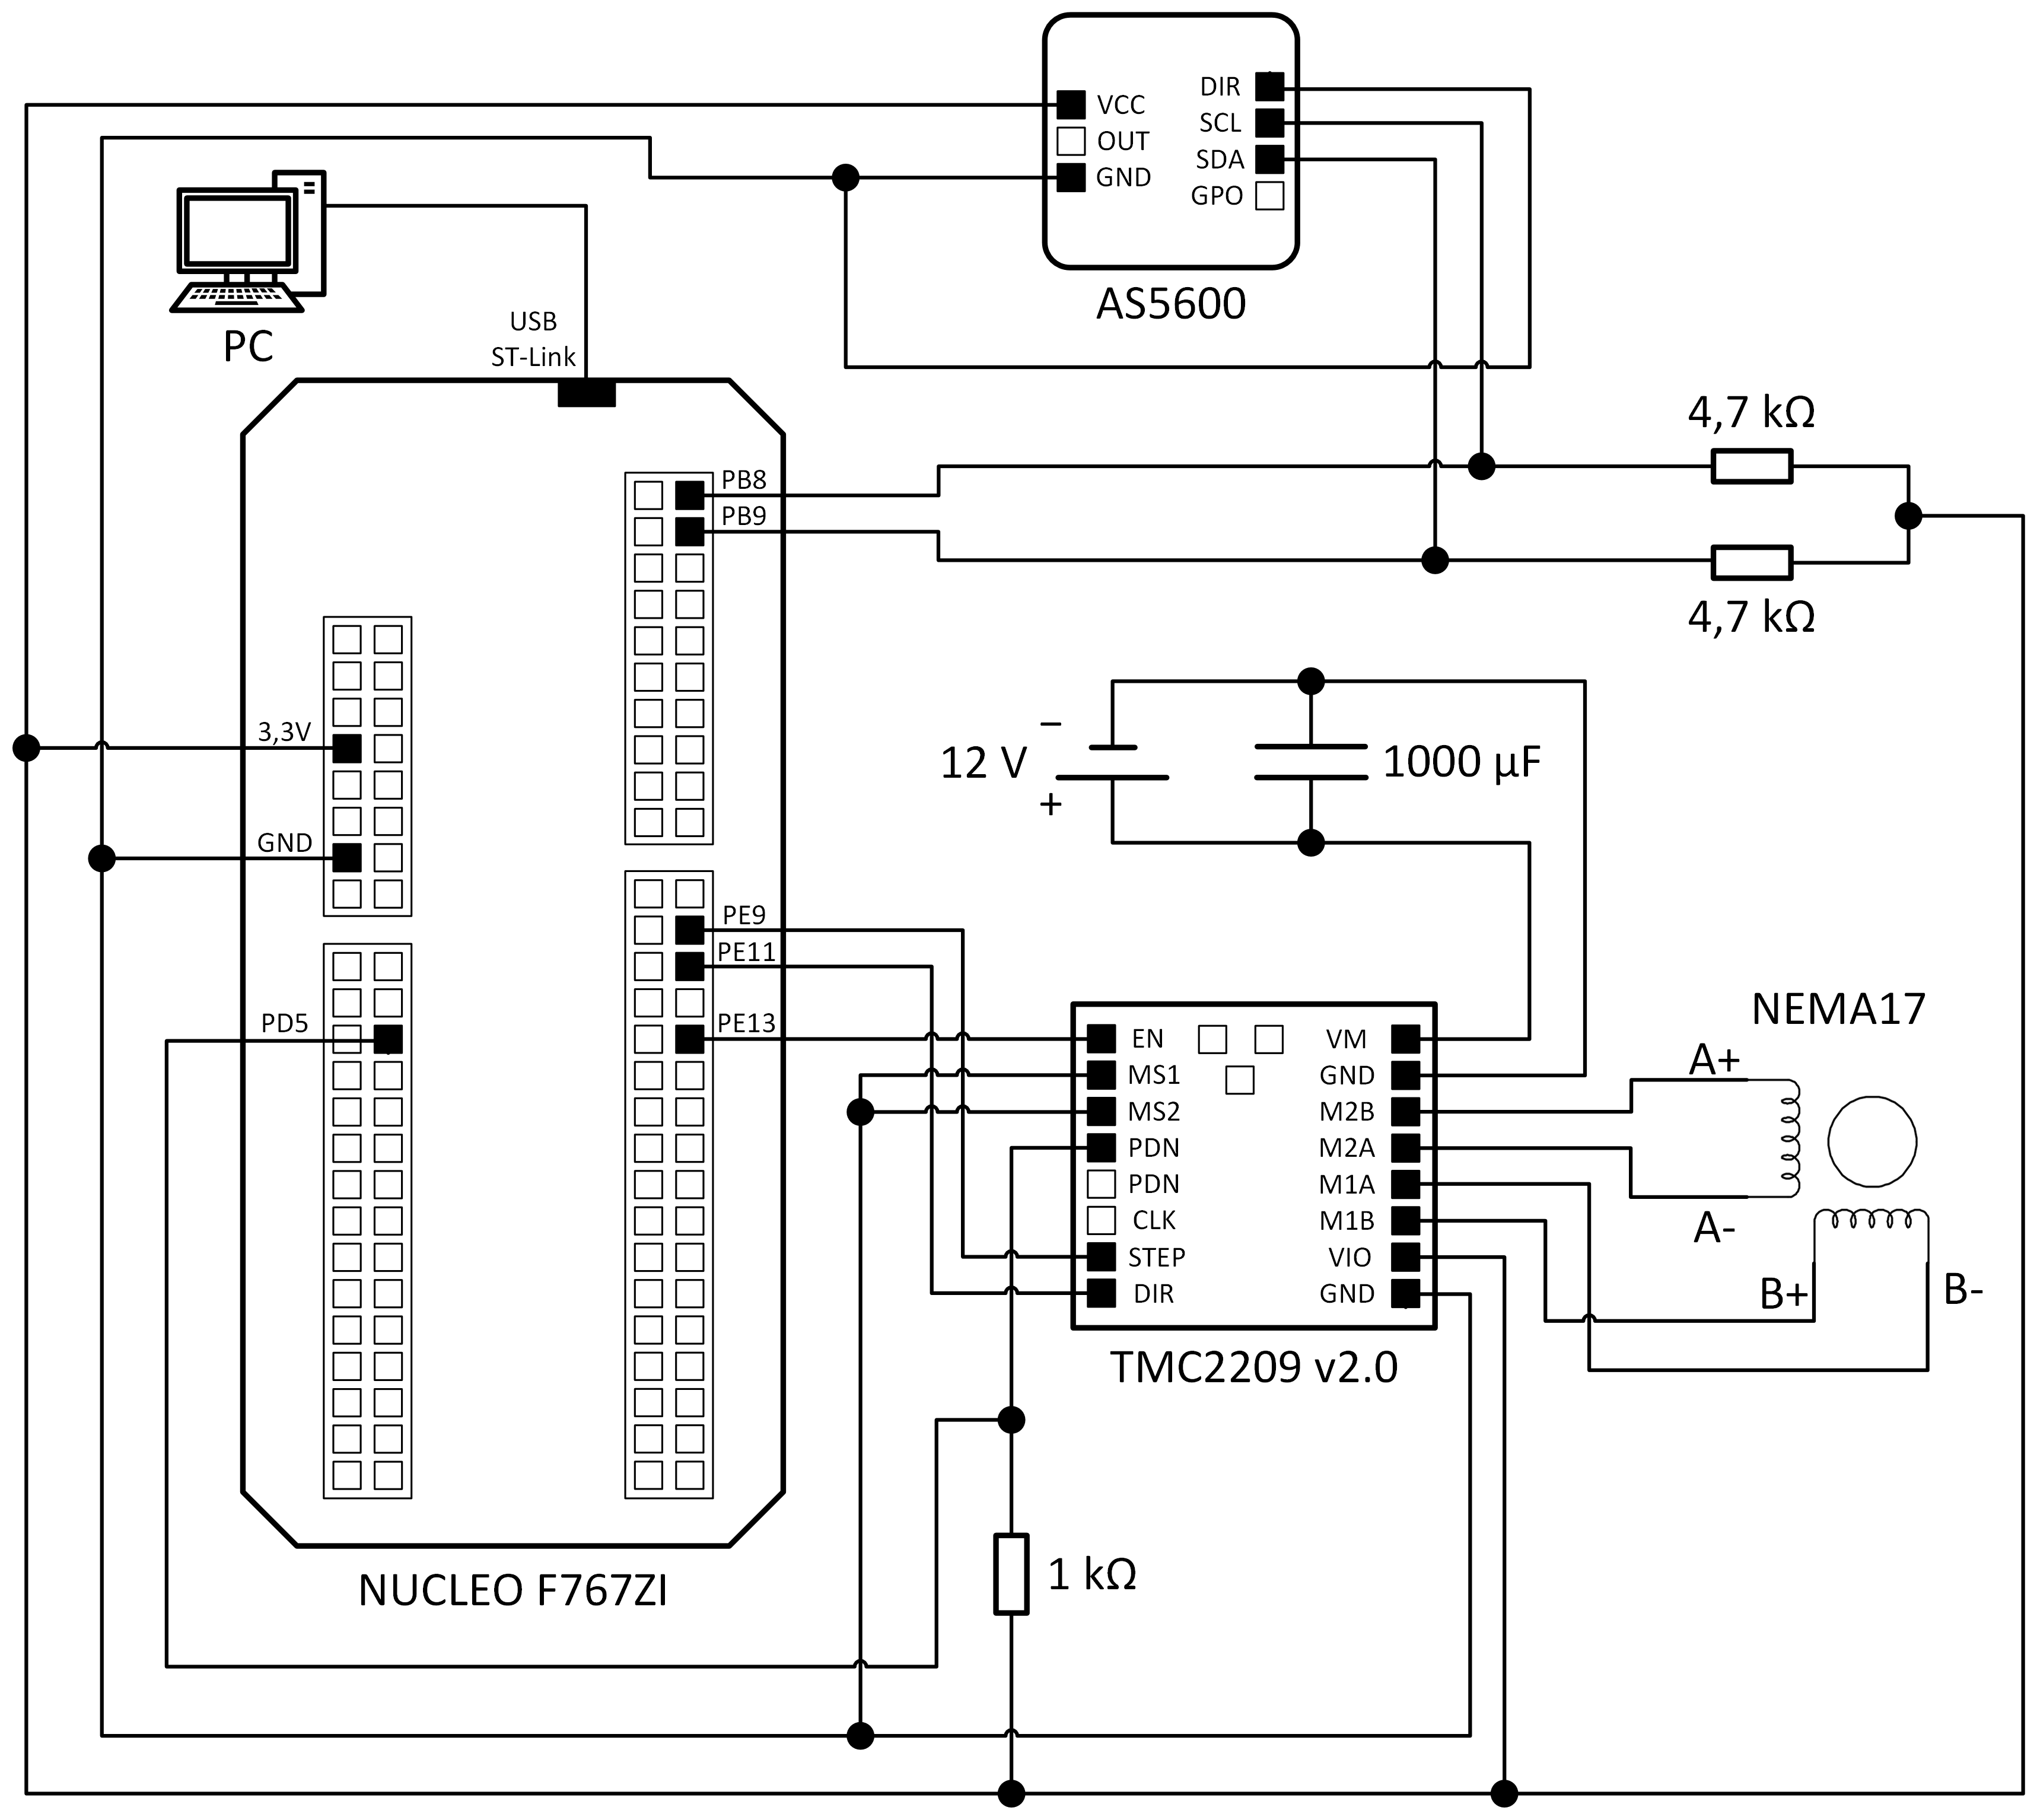
\includegraphics[width=1\linewidth]{Abbildung/SimReg_Schaltplan.png}
    \caption{Schaltplan des Prüfstands}
    \label{fig:Schaltplan}
\end{figure}


